\chapter{Introduction to Wireless Sensor Networks} \label{chap:IntroWSN}
This chapter presents a brief introduction to Wireless Sensor Networks (WSNs).
Additionaly, it describes the reference WSN protocol stack used as part of this
work, and provides a short overview of WSN routing techniques.

\section{Sensor Nodes} \label{subsec:sensornodes}
WSNs are, as described earlier (see Chapter \ref{chap:Intro}), networks of sensor
nodes, and are typically deployed randomly in a possibly large area where
phenomena are required to be monitored.

As presented in Figure \ref{Fig:SensorNodeArch}, a sensor node consists of
the following elements:
\begin{itemize}
  \item \emph{Sensing unit}, which is comprised of a number of sensors and
  analog-to-digital converters. 
  \item \emph{Transceiver}, which facilitates node-node communication using 
a variety of techniques.
  \item \emph{Processing unit}, that comprises a 
microcontroller/microprocessor that performs processing, and is associated with 
a storage unit.
  \item \emph{Power unit}, which provides the energy required to run the sensor node, and can use chemical 
batteries or power scavenging units such as solar cells.
\end{itemize}

\begin{figure}[h]
\centering
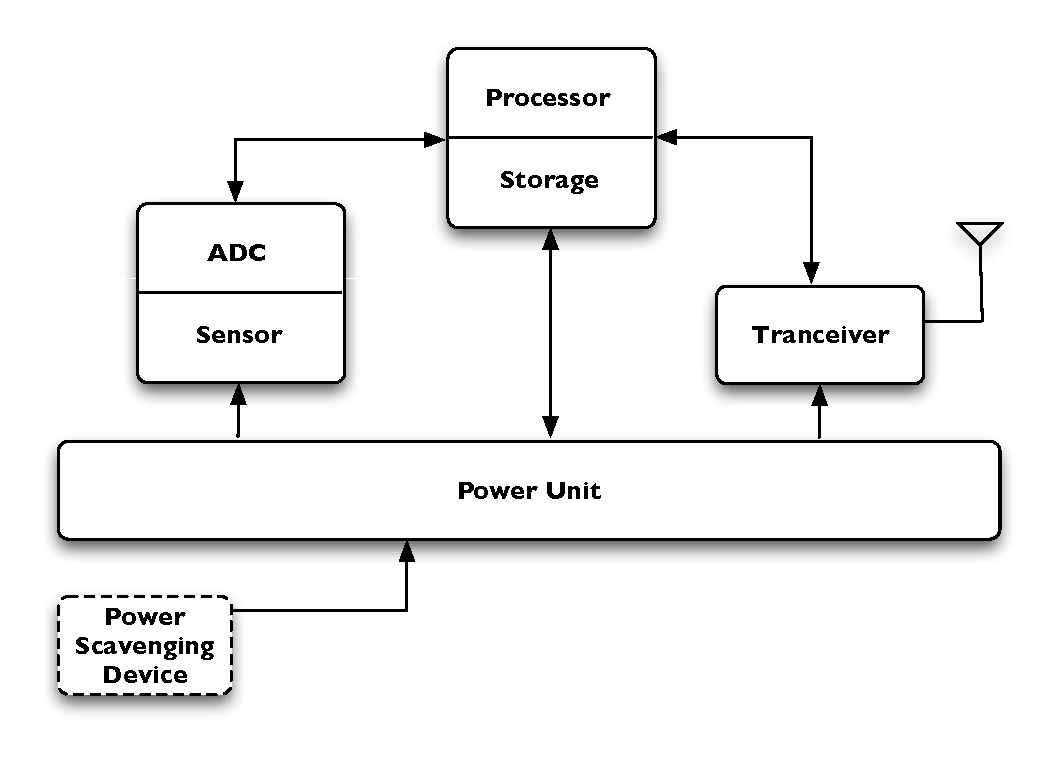
\includegraphics[scale=0.65]{img/SensorNodeArch.eps} 
\caption[Architecture of a sensor node] {Architecture of a sensor node (adapted from \cite{SensorSurveyAkyildiz:2002}).}
\label{Fig:SensorNodeArch}
\end{figure} 

Due to the small size of the devices, sensor nodes have a number of constraints
which affect the WSN built on top of it. These include \cite{yao:qps}:
\begin{itemize}
  \item \emph{Power consumption constraint,} due to the fact that sensor nodes
  have limited energy supply. Therefore, energy conservation is the main concern when
  WSN applications are implemented.
  \item \emph{Computation restriction,} caused by the limited memory
  capacity and processing power available on the sensor node. This places
  serious limitations on the use of data processing algorithms on a sensor node.
  
  \item \emph{Communication constraint,} as a result of the minimal bandwidth available and a
  limited Quality of Service (QoS) provided by the sensor node's hardware. 
\end{itemize}

Additionally, as the deployment of sensor nodes in the WSNs should be
cost-effective, the cost of a single device is a supplementary constraint.

A WSN is self-organising system, given the random nature of the deployment. Its
topology is subject to change, and therefore, sensor nodes should be capable of
dealing with changes of this kind in order to cope with hostile operating
conditions, the failure-prone nature of sensor nodes and the possibility of
redeployment of additional sensor nodes at any time during operation.

\section{WSN Protocol Stack} \label{sec:WSNProtStack}

The WSN protocol stack presented in \cite{SensorSurveyAkyildiz:2002} is an
adaptation of a generic protocol stack \cite{ComputerNetworksTannenbaum:2003}.


\begin{figure}[h]
\centering
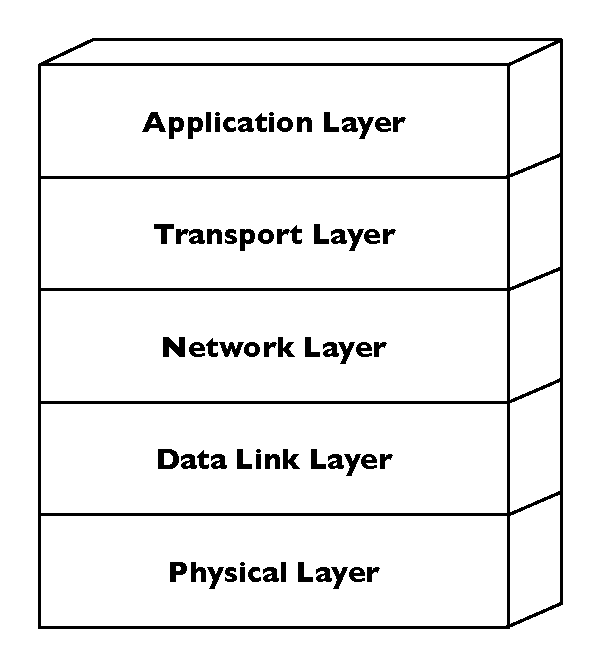
\includegraphics[scale=0.65]{img/ProtStack.eps}
\caption[WSN protocol stack]{WSN protocol stack (reproduced from \cite{SensorSurveyAkyildiz:2002})}
\label{Fig:ProtStack}
\end{figure}

According to \cite{SensorSurveyAkyildiz:2002} the WSN protocol stack consists
of the following layers:

\begin{itemize}
\item \emph{Physical Layer}, which provides the transmission of data over the physical transmission medium.
\item \emph{Data Link Layer}, which deals with power-aware Medium Access Control (MAC) protocols that minimise collisions and transceiver on-time.
\item \emph{Network Layer}, which is primarily responsible for
routing data across the network.
\item \emph{Transport Layer}, which provides reliable delivering of data and
supports error checking mechanisms.
\item \emph{Application Layer}, where the application software resides.
\end{itemize}


\section {Routing in WSNs}

The existing constraints of the sensor nodes influence the design of routing
protocols, and these limitations have to be overcome in order to provide
efficient communication in WSNs \cite{routing:2004}.

Routing algorithms may be classified on the basis of the organisation of
the network structure used. Routing algorithms are thus primarily classified into being either:
\begin{itemize}
\item \emph{Flat}, where every node plays the same role, 
\item \emph{Hierarchical}, where the network is organised into physically
defined clusters,
\item \emph{Location-based}, where positioning information is used to direct traffic to a given physical subset of
the network.
\end{itemize}

Additionally, depending on how the source finds a route to the destination
routing protocols can be split into three categories \cite{routing:2004}:
\begin{itemize}
	\item \emph{Proactive}, when all routes are known before they are used
	\item \emph{Reactive}, when route is computed on demand 
	\item \emph{Hybrid}, which uses a combination of the two techniques above.
\end{itemize}

The LN routing algorithm that is principal to this work may be considered an
extension of a location-based, hybrid routing algorithm, as logical predicates
are used to direct traffic to a specific \emph{logical} subset of the network. A more
detailed discussion of the LN mechanism may be found in
Chapter \ref{chap:background}.

\section{Summary}
This chapter presented an introduction to WSNs and discussed in detail the 
sensor nodes that constitute them. This was followed by a description of the WSN
protocol stack. The chapter concluded with a classification of
existing WSN routing mechanisms, and placed the techniques and concepts used during the course of
this work within this classification.


